\documentclass[12pt,a4paper,utf8x]{report}
\usepackage [frenchb]{babel}

% Pour pouvoir utiliser
\usepackage{ucs}
\usepackage[utf8x]{inputenc}

\usepackage{url} % Pour avoir de belles url
\usepackage {geometry}

% Pour mettre du code source
\usepackage {listings}
% Pour pouvoir passer en paysage
\usepackage{lscape}

% Pour pouvoir faire plusieurs colonnes
\usepackage {multicol}
% POur crééer un index
\usepackage{makeidx}
\makeindex

% Pour les entetes de page
% \usepackage{fancyheadings}
%\pagestyle{fancy}
%\renewcommand{\sectionmark}[1]{\markboth{#1}{}}
%\renewcommand{\subsectionmark}[1]{\markright{#1}}

% Pour l'interligne de 1.5
\usepackage {setspace}
% Pour les marges de la page
\geometry{a4paper, top=2.5cm, bottom=3.5cm, left=1.5cm, right=1.5cm, marginparwidth=1.2cm}

\parskip=5pt %% distance entre § (paragraphe)
\sloppy %% respecter toujours la marge de droite

% Pour les pénalités :
\interfootnotelinepenalty=150 %note de bas de page
\widowpenalty=150 %% veuves et orphelines
\clubpenalty=150

%Pour la longueur de l'indentation des paragraphes
\setlength{\parindent}{15mm}



%%%% debut macro pour enlever le nom chapitre %%%%
\makeatletter
\def\@makechapterhead#1{%
  \vspace*{50\p@}%
  {\parindent \z@ \raggedright \normalfont
    \interlinepenalty\@M
    \ifnum \c@secnumdepth >\m@ne
        \Huge\bfseries \thechapter\quad
    \fi
    \Huge \bfseries #1\par\nobreak
    \vskip 40\p@
  }}

\def\@makeschapterhead#1{%
  \vspace*{50\p@}%
  {\parindent \z@ \raggedright
    \normalfont
    \interlinepenalty\@M
    \Huge \bfseries  #1\par\nobreak
    \vskip 40\p@
  }}
\makeatother
%%%% fin macro %%%%

%Couverture

\title
{
	\normalsize{Lycée Jean Bart - Dunkerque\\
	2011-2012}\\
	\vspace{15mm}
	\Huge{Note de synthèse}
}
\author{\bsc{Stechele} Julien\\
	\vspace{45mm}
}

\date{
	\normalsize{IdentIt\\
    1294 rue Achille \bsc{Pérès}\\
	Petite-Synthe\\
	\vspace{5mm}
    Tuteur de stage : M.\bsc{Anselin}\\
	Maitre de stage : M.\bsc{Dubourg}
	}
}

\begin{document}

\maketitle

\chapter*{Remerciements} % (fold)

Je tiens à remercier :
\begin{itemize}
\item M.\bsc{Dubourg} pour le suivi qu'il m'a apporté pendant toute la durée du
stage, le temps qu'il m'a consacré pour m'initier à la programmation orienté
objet, les astuces techniques pour développer plus rapidement ainsi que
l'enseignement des habitudes propres à l'entreprise.
\item La société IdentIt pour avoir accepté ma candidature, j'espère avoir
été à la hauteur de leurs attentes.
\item L'équipe de développeurs pour m'avoir aiguiller quand j'étais en
détresse.
\item L'équipe enseignante pour nous avoir appris les fondements du
développement et l'univers informatique tout autour qui en découle.
\end{itemize}
% chapter Remerciements (end)


\tableofcontents
\clearpage

% Pour avoir un interligne de 1,5
\begin{onehalfspace}

\chapter{Introduction}

Je m'appelle Julien \bsc{Stechele}, je suis actuellement en BTS\,
\footnote{\emph{Brevet de Technicien Supérieur.}} informatique de gestion
option développeur d'applications et dans le cadre de mes études j'ai la chance
d'effectuer deux stages durant cette formation. Mon stage de première année s'est déroulé du 16 mai 2011 au 8 juillet 2011 dans la société \emph{IdentIt}
qui se situe à Petite-Synthe. C'est une SARL\, \footnote{\emph{Société à
responsabilité limitée.}} de quatre personnes, M.\bsc{Dubourg} et
M.\bsc{Lesage} sont les fondateurs de cette structure, le premier s'occupant de
la partie technique entant que chef de projet, le second s'attelant de la
partie gestion de l'entreprise. Ils sont accompagnés par deux développeurs,
l'un travaillant sur la partie application sur Windows Mobile \copyright,
l'autre sur la partie internet.

Mon premier travail consistait à développer sur la partie web un utilitaire de
comparaison de base de données qui permetterait d'améliorer le suivi des mises
à jour d'une base obsolète à partir d'une base de référence et aussi de fournir
les requêtes permettant cette mise à jour. Mon deuxième travail était de mettre
en place un nouvel outil de gestion de version de code source plus évolué que
l'existant.

Le premier jour en entreprise fut un peu spécial pour moi. En effet, mon
entretien s'étant passé un vendredi après-midi, seul les gérants de
l'entreprise était présent, du coup cela a été pour moi l'occasion de
rencontrer les deux développeurs, Cyril\, \footnote{Titulaire d'un BTS IG à
Jean \bsc{Bart} promotion 2009.} tout juste arrivé dans l'entreprise et
Ludovic, développeur expérimenté qui a de nombreuses années de programmation
derrière lui.

Cette note de synthèse suivant un plan spécifique, les événements ne se sont
pas passés dans l'ordre exacte dans lequel je les raconte. En effet, à cause
des difficultés rencontrées et des problématiques nouvelles donné en cours de
stage, je suis beaucoup passé d'une réalisation à une autre.

\clearpage


\chapter{La gestion de version}

\section{Git : le gestionnaire de code source}

Les logiciels de gestion de versions ou VCS\, \footnote{\emph{Version Control
System.}} sont utilisés principalement par les développeurs. En effet, ils sont
quasi exclusivement utilisés pour gérer des codes sources, car ils sont
capables de suivre l’évolution d’un fichier texte \emph{ligne de code par ligne de
code.} Ces logiciels sont fortement conseillés pour gérer un projet
informatique.

Ils retiennent qui a effectué chaque modification de chaque fichier et
pourquoi. Ils sont par conséquent capables de dire qui a écrit chaque ligne de
chaque fichier et dans quel but ; si deux personnes travaillent simultanément
sur un même fichier, ils sont capables d’assembler (de fusionner) leurs
modifications et d’éviter que le travail d’une de ces personnes ne soit écrasé.

Ces logiciels ont donc par conséquent deux utilités principales :
\begin{itemize}
    \item suivre l’évolution d’un code source, pour retenir les modifications
effectuées sur chaque fichier et être ainsi capable de revenir en arrière en
cas de problème ;
    \item travailler à plusieurs, sans risquer de se marcher sur les pieds.
Si deux personnes modifient un même fichier en même temps, leurs modifications
doivent pouvoir être fusionnées sans perte d’information.
\end{itemize}

Chaque utilisateur possède une copie du code source ainsi que toutes les
versions précédentes de celui-ci, ce qui n'est pas le cas de l'existant. La
figure \ref{workflow} en  page \pageref{workflow} illustre bien le
fonctionnement global de Git.

\begin{figure}
\begin{center}
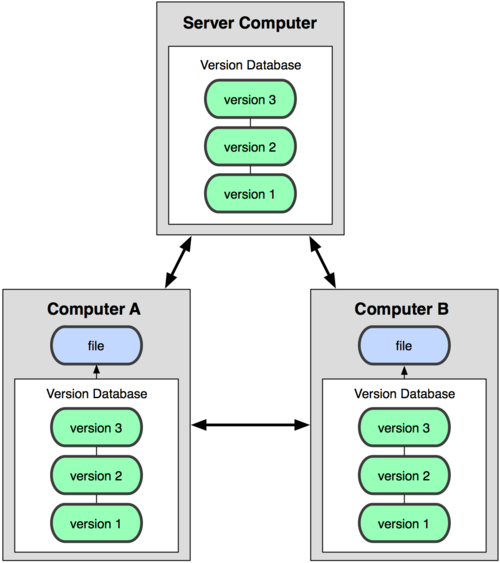
\includegraphics[scale=0.8]{images/workflow.png}
\caption{Le serveur sert de point de rencontre entre les développeurs et possède
lui aussi l’historique des versions.}
\label{workflow}
\end{center}
\end{figure}

\subsection{Les rudiments}

\emph{Un commit} correspond à un enregistrement des modifications dans le
temps. Admettons un fichier qui contient un paragraphe, si nous ajoutons un
deuxième paragraphe, le fichier sera considéré comme modifié par Git\,
\footnote{Créé par Linus Torvalds, qui est entre autres l'homme à l'origine de
Linux. Il est de type distribué.}, pour enregistrer la modification on effectue
un commit. L'analogie la plus simple est celle des jeux vidéos où vous
sauvegardez votre progression à chaque étape franchie.

\emph{Une branche} représente une \og copie virtuelle \fg{} du dossier
contenant les fichiers sources. En effet, il est possible de cloner
virtuellement un dépôt et de basculer de l'original à la copie pour développer,
par exemple, sur la branche principale les nouvelles fonctionnalités et sur
l'autre branche les corrections d'erreurs comme nous le montre la figure
\ref{branches}.

\begin{figure}
\begin{center}
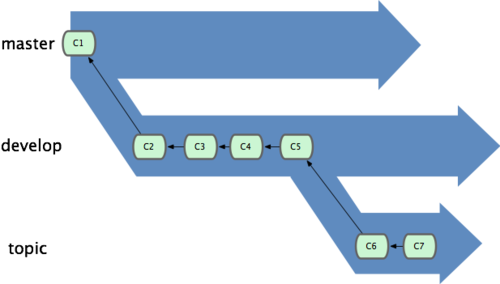
\includegraphics[scale=0.8]{images/branches.png}
\caption{master, develop et topic, trois branches d'un même dépôt.}
\label{branches}
\end{center}
\end{figure}

\emph{La fusion} est l'opération de rassemblement des deux branches en une,
c'est-à-dire dans le cas précédent de regrouper les corrections d'erreurs avec
les nouvelles fonctionnalités.

Les fondamentaux ayant été acquis, j'ai trouvé plusieurs solutions à la
problématique principale qui est la suivante : \newline

Peut-on fusionner des branches tout en choisissant de ne pas fusionner
tout les commits ? \newline

\begin{itemize}
    \item Tout dabord la commande \texttt{git chery-pick nomducommit} permet
    de \og cueillir \fg{} le commit que l'on veut fusionner.
    \item Ensuite on peut aussi rassembler les deux branches puis exécuter la
    commande \texttt{git revert nomducommit} pour inverser les modifications
    du commit après la fusion.
    \item Enfin faire trois branches distinctes pour ne pas avoir à faire les
    opérations ci-dessus\, \footnote{Cette solution à été choisie.}.
\end{itemize}

Git répondant au besoin de l'entreprise, il a fallu que j'effectue des
recherches pour que la migration Subversion\, \footnote{Le logiciel de gestion
de versions le plus utilisé à l'heure actuelle. Il est de type centralisé.}
vers Git se fasse sans perte.

\subsection{L'installation} % (fold)

À peu près au milieu du stage, nous nous sommes heurtés à un problème
technique. Le serveur de l'entreprise ne contenait pas de version récente de
Git. En sachant que celui-ci est mutualisé\, \footnote{L'hébergement mutualisé
est un concept d'hébergement internet destiné principalement à des sites web,
dans un environnement technique dont la caractéristique principale est d'être
partagé par plusieurs utilisateurs. L'administration du ou des serveurs est
assurée par un intervenant tiers tel qu'OVH.}, nous n'avions pas les
autorisations nécessaires pour installer une nouvelle version.

Les logiciels libres sont réputés pour être rétro-compatibles, mais en toute
logique il ne dispose pas des nouveautés sans les mettre à jour. Le problème
est qu'on ne pouvait pas modifier des branches distantes dites \og de suivi
\fg{}. Cette fonctionnalité permet à plusieurs développeurs de travailler en
même temps sur une branche différente de celle par défaut, par exemple pour
expérimenter de nouvelles implémentations à plusieurs. À ce moment-là j'ai été
très déçu et pensais mon travail inutilisable. Cependant, mes efforts n'ont pas
été vain puisque M.\bsc{Dubourg} après quelques recherches, a trouvé sur
internet un utilisateur ayant réussi à installer Git sur un serveur mutualisé.
Nous n'avions pas les droits d'accès aux dossiers des programmes mais rien ne
nous empêchait de compiler Git à partir des sources pour nous permettre de
créer en local le logiciel\, \footnote{Le problème ne se serait pas posé si
j'avais lu le chapitre traitant de la compilation dans mon livre Linux, je n'ai
découvert cette méthode qu'après le stage\dots}. Ceci étant fait, en
redéfinissant la variable système qui stocke les chemins des applications, nous
avons pu utiliser notre compilé dernier cri.

% section L'installation (end)

\subsection{Le passage fatidique} % (fold)

Trois jours avant mon départ, le grand déménagement s'impose. Toute la partie
étude et confection du tutoriel Git prend forme car j'ai basculé tous les
projets qui étaient au préalable sur Subversion vers Git tout en gardant
l'historique des changements provenant de SVN. Après quelques recherches, une
commande Git m'a permis de répondre à ce besoin.

\begin{lstlisting}
git-svn clone http://svn/repo/here/trunk
\end{lstlisting}
% section Le passage fatidique (end)

\section{Les utilitaires} % (fold)

Nous avons longuement discuté sur le côté technique de Git. En effet cet outil
est à la base un logiciel libre provenant de Linux et n'a pas d'interface
graphique, ce choix est établi sur le fait qu'un développeur n'a pas forcément
besoin de cela pour travailler\, \footnote{Sans nul doute que pour un
graphiste, une souris est un élément indispensable pour ses créations, mais pas
pour produire du code.} et aussi que ce logiciel regorge de fonctionnalités et
donc très difficile à simplifier à travers une interface ne pouvant fonctionner
qu'avec une souris. L'équipe n'étant pas très férue de ligne de commande et le
logiciel TortoiseGit reprenant que les fonctions essentielles de Git, il a
fallu que je conçois des petits programmes qui fonctionnent en un clic pour
simplifier les choses répétitives.

% section Introduction (end)

\subsection{Lister les dépôts du serveur}

Mon travail suivant consistait à lister les dépôts Git dans une page PHP\,
\footnote{\emph{Hypertext Preprocessor} est un langage de scripts libre
principalement utilisé pour produire des pages Web dynamiques.}. Le serveur OVH
centralise les codes sources de la société, les développeurs, eux doivent
récupérer une copie des dossiers pour pouvoir travailler dessus. Seulement,
lancer FilleZilla\, \footnote{FileZilla est un logiciel gratuit qui permet de
se connecter à distance sur un serveur pour y télécharger des fichiers.} pour
connaître les noms des répertoires Git puis recopier le bon lien hypertexte
avec le bon chemin d'arborescence est une tâche fastidieuse.  J'ai donc, à
l'aide de mes connaissances en système UNIX, créé un script qui analyse un
dossier défini et qui liste les différents dépôts tout en leurs mettant les
bonnes adresses de téléchargement en préfixe. Du coup, un simple copier-coller
du lien du dépôt voulu dans tortoiseGit suffit pour cloner. Gain de
productivité et de simplicité réunie.

\begin{figure}
\begin{center}
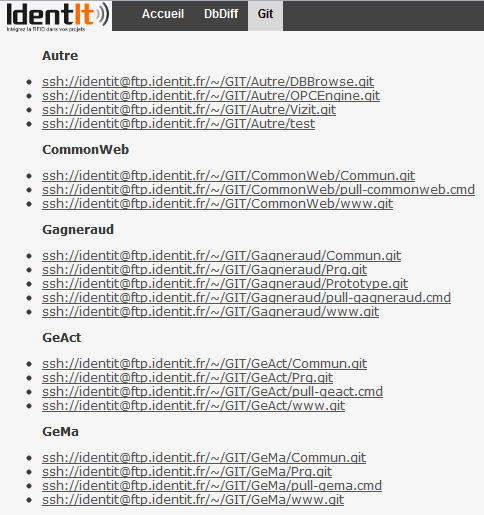
\includegraphics[scale=0.5]{images/repo.png}
\caption{La liste des dépôts cliquables.}
\label{repo}
\end{center}
\end{figure}

% section Mise à jour distante automatique (end)

\subsection{Mise en production automatique} % (fold)

Une fois que les développeurs sont satisfaits de leurs modifications, ils
doivent mettre à jour le dépôt distant pour partager leurs travaux. Une fois
les modifications validées par le chef de projet, celui-ci doit mettre en ligne
sur le dépôt de production. J'ai créé un script Batch \og modèle \fg{} pour
que cela ce fasse en un clic.\\

pull-dossier.cmd :
\begin{lstlisting}
set PATH=%HOMEPATH%;%PATH%
plink identit@ftp.identit.fr -l identit -pw MOTDEPASSE
"cd LEDOSSIER;
git pull;
exit;"
\end{lstlisting}

% section Mise en production automatique (end)

\subsection{Mise à jour locale automatique} % (fold)

Les développeurs possèdent des clones des dépôts distants\, \footnote{Ils se
trouvent tous sur le serveur OVH qui sert de point de rencontre comme nous
l'avons vu.} en local pour bien évidemment maintenir le code source. Le fait
qu'il y ait une multitude de dépôts implique une mise à jour des clones locaux
pour récupérer les modifications des autres développeurs ce qui est très
répétitif. J'ai donc créé un script Batch\, \footnote{Désigne un fichier qui
contient une suite de commandes qui seront traitées automatiquement par
Windows\, \copyright.} qui parcourt tous les dossiers englobant les sources des
dépôts et les mets à jour. Pour cela j'ai parcouru la documentation de la
console windows\, et ça n'a pas été évident du tout. Pour l'anecdote, je devais
à partir de mon MacBook\, \footnote{Système de type UNIX.}, lancer une machine
virtuelle Windows\, \footnote{À partir du logiciel VirtualBox.} pour créer mon
script Batch qui s'execute en console, et qui lance enfin un terminal Linux
pour faire la mise à jour\dots\\

pullall.cmd :
\begin{lstlisting}
"C:\Program Files\TortoiseGit\bin\pageant.exe"
C:%HOMEPATH%\.ssh\id_rsa.ppk
"C:\Program Files (x86)\git\bin\sh.exe" --login -i -c
"for i in $(find . -maxdepth 2 -mindepth 2 -type d);
do
    cd $i;
    echo $i;
    git remote -v;
    git pull; cd ../..;
done"
\end{lstlisting}

\clearpage


\chapter{Script de comparaison}

N'ayant pas de notions de programmation orientée objet\, \footnote{Ce qui sera
enseignée en deuxième année.} je n'ai pas pu rejoindre les développeurs de
l'entreprise dans l'application qu'ils développaient, cela dit on m'a confié
une tâche annexe qui est la comparaison des bases de données. Le schéma
\ref{bdd} en page \pageref{bdd} nous en illustre une structure basique.

\begin{figure}
\begin{center}
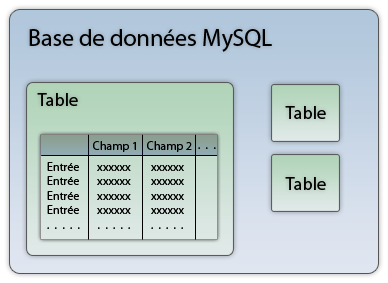
\includegraphics[scale=0.5]{images/bdd.png}
\end{center}
\caption{Un schéma de base de données simple.}
\label{bdd}
\end{figure}

Le besoin premier de ce script est de consulter les différences de structure
qui existent entre une base de référence est une base à mettre à jour. Dans le
cas de l'entreprise, il permettrait un suivi des mises à jour des applications
fournies au client et pour moi, m'initier à la programmation orientée objet\,
\footnote{La programmation orientée objet est un paradigme de programmation qui
consiste à utiliser des objets ; un objet représente un concept, une idée ou
toute entité du monde physique, comme une voiture, une personne ou encore une
page d'un livre.} dès le premier stage.

\section{Le départ}

À l'aide d'un cours sur internet, j'ai commencé à créer ma première classe.
Cette classe après instanciation représenterait l'objet \og base de données
\fg{} sous forme de tableau. L'image \ref{obj} qui ce trouve en page
\pageref{obj} est plus parlante.

\begin{figure}
\begin{center}
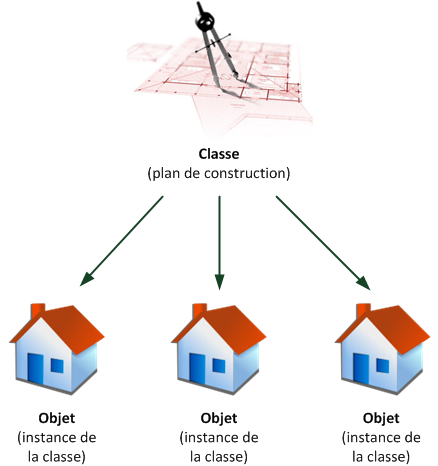
\includegraphics[scale=0.5]{images/objet.png}
\end{center}
\caption{Un plan à partir duquel on crée des objets.}
\label{obj}
\end{figure}

Passer de la programmation fonctionnelle\, \footnote{La programmation
fonctionnelle est un paradigme de programmation qui repose sur l'utilisation
majoritaire des fonctions et procédures.} à l'objet fut vraiment difficile. Me
rendant compte que je bloquais énormément, je fis des recherches sur internet
pour trouver un programme équivalent sur lequel je me suis appuyé pour
commencer. M.\bsc{Dubourg} m'a mis sur la voie en me disant d'utiliser des
classes et des méthodes toutes prêtes de l'entreprise ce qui me fit gagner
beaucoup de temps, car je savais pas comment transcrire une structure de base de données en objet.

Pour utiliser les sources de la société, j'ai dû mettre en place un répertoire
de travail et récupérer les sources via leur ancien gestionnaire de version de
code source. Ceci étant fait il s'agissait maintenant de réussir à faire
fonctionner le site web principal en local sur ma machine. Comme mon logiciel
MAMP\, \footnote{\emph{Macintosh Apache MySQL PHP.} est une combinaison de
logiciel.} m'affichait plein d'erreurs, j'ai décidé d'installer manuellement
chacun des logiciels présents dans celui-ci. Même après cette manipulation le
problème n'avait pas disparu, mon tuteur de stage m'est venu en aide après de
longues heures à chercher en vain. Le problème était tout d'abord au niveau de
la configuration de PHP, qui affichait tous les avertissements de manière trop
stricte, ce qui entravait le lancement de la page principale. Il était aussi au
niveau du cache de mon navigateur. En effet, j'ai du vider celui-ci pour faire
enfin apparaitre le site proprement. De nombreuses heures de recherche juste à
cause d'un cache internet non vidé fut extrêmement frustrant \ldots{}

\section{Comparaison des tables}

Il a fallu dans un premier temps que je recherche comment extraire le nom d'une
base ainsi que le nom de ses tables. La réponse à cette question est dans la
documentation de MySQL. Une base de données est fournit à l'installation et
s'appelle \og information schéma \fg{} . En résumé, c'est une base de données
qui contient toutes les autres.

Ensuite, j'ai transformé le programme procédural sur plusieurs semaines en
objet, le fait de passer par cette étape intermédiaire m'a permis d'abord de
résoudre le problème algorithmiquement, puis de me consacrer sur la façon de
l'écrire.

La requête récupérant les données utiles, j'ai dû concevoir un algorithme
capable de comparer les deux tableaux d'objets par rapport à leurs noms :
\begin{itemize}
    \item Si la base de données de référence a une table qui n'est pas dans
    la base de données à mettre à jour, on l'ajoute ;
    \item Si la base de données à mettre à jour contient une table qui n'est
    pas dans la base de données de référence, on l'enlève ;
    \item Si les tables comparées sont toutes les deux dans les bases de
    données, on compare l'intérieur des tables.
\end{itemize}

J'ai dû revoir mon algorithme plusieurs fois, car la fonction de comparaison de
chaine de caractère \texttt{strnatcmp} compare les mots comme un humain le
ferait, alors que mySQL trie les tables de manière binaire grâce aux codes
ASCII\, \footnote{\emph{American Standard Code for Information Interchange.} ou
\og Code américain normalisé pour l'échange d'information \fg{} est la norme de
codage de caractères en informatique la plus connue, la plus ancienne et la
plus largement compatible. ASCII contient les caractères nécessaires pour
écrire en anglais.} des caractères ce qui faisait que la première fonction
fonction donnait des résultats erronés comme le montre le tableau \ref{tab}.

\begin{table}
\begin{center}
\begin{tabular}{|c|c|}
\hline
\textbf{Tri de chaînes standard} & \textbf{Tri de chaînes ordre naturel} \\
\hline
[0] = img1.png & [0] = img1.png \\
\hline
[1] = img10.png & [1] = img2.png \\
\hline
[2] = img12.png & [2] = img10.png \\
\hline
[3] = img2.png & [3] = img12.png \\
\hline
\end{tabular}
\caption{La différence entre les tris de chaînes.}
\label{tab}
\end{center}
\end{table}

\section{Comparaison des champs}

J'étais dans la situation des tables ayant les mêmes noms, il fallait que je
compare le contenu à partir du nom des champs. Il ne m'a pas fallut longtemps
pour comprendre que l'algorithme était exactement le même, le plus dur étant de
savoir comment j'allais faire pour ne pas me répéter, ce qui a bloqué
énormément mon avancé pour pas grand-chose. M.\bsc{Dubourg} constatant que je
stagnais, m'a conseillé de faire comme j'avais appris plutôt que d'essayer de
faire de la POO\, \footnote{\emph{Programmation Orientée Objet.}}.  Une fois le
script fonctionnel, qui était cependant mal optimisé et peu lisible, mon tuteur
me guida avec des explications poussées sur la marche à suivre. De fil en
aiguille le code source passa d'environ trois-cent cinquante lignes à cent
cinquante.

Ensuite, je devais comparer le contenu des champs des tables lorsque les champs
parcourus avait le même nom. Je comparais tout simplement le contenu des champs
pour connaitre l'issue finale, à savoir que je ne pouvais pas décider si les
tables étaient similaire sans avoir balayé tous les champs et toutes les
caractéristiques de ceux-ci.

\section{Affichage du résultat}

Après tout ceci fini et optimisé, j'implémente une nouvelle fonctionnalité qui
permettrait d'afficher un texte lisible qui énonce les différences des deux
bases de données. En fonction des résultats obtenus, je génère des balises HTML\,
\footnote{L’ \emph{Hypertext Markup Language} est un langage de balisage conçu
pour représenter les pages web.} et du texte pour que cela soit compréhensible
à l'utilisateur. Ceci étant fait assez rapidement je suis passé à la génération
des requêtes SQL\, \footnote{\emph{Structured Query Language} est un langage
informatique normalisé qui sert à effectuer des opérations sur des bases de
données.} permettant de mettre à jour la base obsolète depuis la base de
référence. C'est à ce stade que j'ai constaté que je ne pourrais pas prendre en
compte les clés étrangères dans mon code à moins de revoir totalement tout le
script. M.\bsc{Dubourg} m'a rassuré sur le fait que l'entreprise n'utilisait pas
le type de base de données myISAM\, \footnote{L'organisation séquentielle
indexée, ou \emph{Indexed Sequential Access Method} en anglais, est un mode
d'organisation des fichiers dans les bases de données.} et que donc aucune de
leurs tables comportait de clé étrangère, cependant les clés primaires
concaténées restent problématiques, car pas imaginer pendant la conception. Nous
avons décidé que la création de ce genre de cas se fera à la main pour ne pas
repartir de zéro.

Après avoir analysé mes méthodes de génération de phrases lisibles et de
requêtes SQL, M.\bsc{Dubourg} m'a présenté un outil nommé \og Smarty \fg{} qui
permet de dissocier la partie traitement de la partie affichage, car il est
vrai que mes méthodes étaient vraiment très sales. Pour résumer, j'écrivais des
chaînes de caractères dans une seule variable en écrivant les noms des tables
ou des champs, en concaténant le tout avec des balises HTML de saut de ligne un
peu n'importe où. J'ai dû parcourir la documentation de Smarty pour comprendre
son fonctionnement, il s'avère que la syntaxe est très particulière mais très
efficace. J'ai terminé par faire de l'agencement sur ma page pour que chaque
ligne lisible par un néophyte soit en face de la ligne traduite en SQL dans un
tableau à deux colonnes.

\clearpage


\chapter{Le titre du chapitre}

\section{Le titre de la section qui va bien}

\subsection{Titre de la sous section}

Ici du texte et du blabla, ce que l'on veut dire et écrire. A remplacer. Ici du texte et du blabla, ce que l'on veut dire et écrire. On peut faire une citation \cite{MotClef4}.
A remplacer. Ici du texte et du blabla, ce que l'on veut dire et écrire. A remplacer. Ici du texte et du blabla, ce que l'on veut dire et écrire. A remplacer. Ici du texte et du blabla, ce que l'on veut dire et écrire. A remplacer. Ici du texte et du blabla, ce que l'on veut dire et écrire. A remplacer.

Ici du texte et du blabla, ce que l'on veut dire et écrire. A remplacer. Ici du texte et du blabla, ce que l'on veut dire et écrire. A remplacer.
Ici du texte et du blabla, ce que l'on veut dire et écrire. A remplacer. Ici du texte et du blabla, ce que l'on veut dire et écrire. A remplacer. Ici du texte et du blabla, ce que l'on veut dire et écrire. A remplacer. Ici du texte et du blabla, ce que l'on veut dire et écrire. A remplacer.

%-- Note de bas de page sur les stades
\protect\footnote{Par exemple, on peut faire un pied de page :
\begin{itemize}
\item avec une liste à puces ;
\item avec une liste à puces ;
\item avec une liste à puces.
\end{itemize}
}
%-- Fin Note de bas de page sur les stades

Ici du texte et du blabla, ce que l'on veut dire et écrire. A remplacer. Ici du texte et du blabla, ce que l'on veut dire et écrire. A remplacer. Ici du texte et du blabla, ce que l'on veut dire et écrire. A remplacer. Ici du texte et du blabla, ce que l'on veut dire et écrire. A remplacer. Ici du texte et du blabla, ce que l'on veut dire et écrire. A remplacer. Ici du texte et du blabla, ce que l'on veut dire et écrire. A remplacer.

\begin{itemize}
\item avec une liste à puces ;
\item avec une liste à puces ;
\item avec une liste à puces.
\end{itemize}

Ici du texte et du blabla, ce que l'on veut dire et écrire. A remplacer. Ici du texte et du blabla, ce que l'on veut dire et écrire. A remplacer. Ici du texte et du blabla, ce que l'on veut dire et écrire. A remplacer. Ici du texte et du blabla, ce que l'on veut dire et écrire. A remplacer. Ici du texte et du blabla, ce que l'on veut dire et écrire. A remplacer. Ici du texte et du blabla, ce que l'on veut dire et écrire. A remplacer.

\subsubsection{Titre de la sous sous section}

Ici du texte et du blabla, ce que l'on veut dire et écrire. A remplacer. Ici du texte et du blabla, ce que l'on veut dire et écrire. A remplacer. Ici du texte et du blabla, ce que l'on veut dire et écrire. A remplacer. Ici du texte et du blabla, ce que l'on veut dire et écrire. A remplacer. Ici du texte et du blabla, ce que l'on veut dire et écrire. A remplacer. Ici du texte et du blabla, ce que l'on veut dire et écrire. A remplacer.

Ici du texte et du blabla, ce que l'on veut dire et écrire. A remplacer. Ici du texte et du blabla, ce que l'on veut dire et écrire. A remplacer. Ici du texte et du blabla, ce que l'on veut dire et écrire. A remplacer. Ici du texte et du blabla, ce que l'on veut dire et écrire. A remplacer. Ici du texte et du blabla, ce que l'on veut dire et écrire. A remplacer. Ici du texte et du blabla, ce que l'on veut dire et écrire. A remplacer.

\subsubsection{Titre de la sous sous section}

Ici du texte et du blabla, ce que l'on veut dire et écrire. A remplacer. Ici du texte et du blabla, ce que l'on veut dire et écrire. A remplacer. Ici du texte et du blabla, ce que l'on veut dire et écrire. A remplacer. Ici du texte et du blabla, ce que l'on veut dire et écrire. A remplacer. Ici du texte et du blabla, ce que l'on veut dire et écrire. A remplacer. Ici du texte et du blabla, ce que l'on veut dire et écrire. A remplacer.

Ici du texte et du blabla, ce que l'on veut dire et écrire. A remplacer. Ici du texte et du blabla, ce que l'on veut dire et écrire. A remplacer. Ici du texte et du blabla, ce que l'on veut dire et écrire. A remplacer. Ici du texte et du blabla, ce que l'on veut dire et écrire. A remplacer. Ici du texte et du blabla, ce que l'on veut dire et écrire. A remplacer. Ici du texte et du blabla, ce que l'on veut dire et écrire. A remplacer.

\subsection{Conclusion}

Ici du texte et du blabla, ce que l'on veut dire et écrire. A remplacer. Ici du texte et du blabla, ce que l'on veut dire et écrire. A remplacer. Ici du texte et du blabla, ce que l'on veut dire et écrire. A remplacer. Ici du texte et du blabla, ce que l'on veut dire et écrire. A remplacer. Ici du texte et du blabla, ce que l'on veut dire et écrire. A remplacer. Ici du texte et du blabla, ce que l'on veut dire et écrire. A remplacer.

Ici du texte et du blabla, ce que l'on veut dire et écrire. A remplacer. Ici du texte et du blabla, ce que l'on veut dire et écrire. A remplacer. Ici du texte et du blabla, ce que l'on veut dire et écrire. A remplacer. Ici du texte et du blabla, ce que l'on veut dire et écrire. A remplacer. Ici du texte et du blabla, ce que l'on veut dire et écrire. A remplacer. Ici du texte et du blabla, ce que l'on veut dire et écrire. A remplacer.

\subsection{Titre de la sous section}

Ici du texte et du blabla, ce que l'on veut dire et écrire. A remplacer. Ici du texte et du blabla, ce que l'on veut dire et écrire. On peut faire une citation \cite{MotClef4}.
A remplacer. Ici du texte et du blabla, ce que l'on veut dire et écrire. A remplacer. Ici du texte et du blabla, ce que l'on veut dire et écrire. A remplacer. Ici du texte et du blabla, ce que l'on veut dire et écrire. A remplacer. Ici du texte et du blabla, ce que l'on veut dire et écrire. A remplacer.

Ici du texte et du blabla, ce que l'on veut dire et écrire. A remplacer. Ici du texte et du blabla, ce que l'on veut dire et écrire. A remplacer.
Ici du texte et du blabla, ce que l'on veut dire et écrire. A remplacer. Ici du texte et du blabla, ce que l'on veut dire et écrire. A remplacer. Ici du texte et du blabla, ce que l'on veut dire et écrire. A remplacer. Ici du texte et du blabla, ce que l'on veut dire et écrire. A remplacer.

\subsection{Titre de la sous section}

Ici du texte et du blabla, ce que l'on veut dire et écrire. A remplacer. Ici du texte et du blabla, ce que l'on veut dire et écrire. On peut faire une citation \cite{MotClef4}.
A remplacer. Ici du texte et du blabla, ce que l'on veut dire et écrire. A remplacer. Ici du texte et du blabla, ce que l'on veut dire et écrire. A remplacer. Ici du texte et du blabla, ce que l'on veut dire et écrire. A remplacer. Ici du texte et du blabla, ce que l'on veut dire et écrire. A remplacer.

Ici du texte et du blabla, ce que l'on veut dire et écrire. A remplacer. Ici du texte et du blabla, ce que l'on veut dire et écrire. A remplacer.
Ici du texte et du blabla, ce que l'on veut dire et écrire. A remplacer. Ici du texte et du blabla, ce que l'on veut dire et écrire. A remplacer. Ici du texte et du blabla, ce que l'on veut dire et écrire. A remplacer. Ici du texte et du blabla, ce que l'on veut dire et écrire. A remplacer.

\clearpage


\chapter{Le titre du chapitre}

\section{Le titre de la section qui va bien}

\subsection{Titre de la sous section}

Ici du texte et du blabla, ce que l'on veut dire et écrire. A remplacer. Ici du texte et du blabla, ce que l'on veut dire et écrire. On peut faire une citation \cite{MotClef4}.
A remplacer. Ici du texte et du blabla, ce que l'on veut dire et écrire. A remplacer. Ici du texte et du blabla, ce que l'on veut dire et écrire. A remplacer. Ici du texte et du blabla, ce que l'on veut dire et écrire. A remplacer. Ici du texte et du blabla, ce que l'on veut dire et écrire. A remplacer.

Ici du texte et du blabla, ce que l'on veut dire et écrire. A remplacer. Ici du texte et du blabla, ce que l'on veut dire et écrire. A remplacer.
Ici du texte et du blabla, ce que l'on veut dire et écrire. A remplacer. Ici du texte et du blabla, ce que l'on veut dire et écrire. A remplacer. Ici du texte et du blabla, ce que l'on veut dire et écrire. A remplacer. Ici du texte et du blabla, ce que l'on veut dire et écrire. A remplacer.

%-- Note de bas de page sur les stades
\protect\footnote{Par exemple, on peut faire un pied de page :
\begin{itemize}
\item avec une liste à puces ;
\item avec une liste à puces ;
\item avec une liste à puces.
\end{itemize}
}
%-- Fin Note de bas de page sur les stades

Ici du texte et du blabla, ce que l'on veut dire et écrire. A remplacer. Ici du texte et du blabla, ce que l'on veut dire et écrire. A remplacer. Ici du texte et du blabla, ce que l'on veut dire et écrire. A remplacer. Ici du texte et du blabla, ce que l'on veut dire et écrire. A remplacer. Ici du texte et du blabla, ce que l'on veut dire et écrire. A remplacer. Ici du texte et du blabla, ce que l'on veut dire et écrire. A remplacer.

\begin{itemize}
\item avec une liste à puces ;
\item avec une liste à puces ;
\item avec une liste à puces.
\end{itemize}

Ici du texte et du blabla, ce que l'on veut dire et écrire. A remplacer. Ici du texte et du blabla, ce que l'on veut dire et écrire. A remplacer. Ici du texte et du blabla, ce que l'on veut dire et écrire. A remplacer. Ici du texte et du blabla, ce que l'on veut dire et écrire. A remplacer. Ici du texte et du blabla, ce que l'on veut dire et écrire. A remplacer. Ici du texte et du blabla, ce que l'on veut dire et écrire. A remplacer.

\subsubsection{Titre de la sous sous section}

Ici du texte et du blabla, ce que l'on veut dire et écrire. A remplacer. Ici du texte et du blabla, ce que l'on veut dire et écrire. A remplacer. Ici du texte et du blabla, ce que l'on veut dire et écrire. A remplacer. Ici du texte et du blabla, ce que l'on veut dire et écrire. A remplacer. Ici du texte et du blabla, ce que l'on veut dire et écrire. A remplacer. Ici du texte et du blabla, ce que l'on veut dire et écrire. A remplacer.

Ici du texte et du blabla, ce que l'on veut dire et écrire. A remplacer. Ici du texte et du blabla, ce que l'on veut dire et écrire. A remplacer. Ici du texte et du blabla, ce que l'on veut dire et écrire. A remplacer. Ici du texte et du blabla, ce que l'on veut dire et écrire. A remplacer. Ici du texte et du blabla, ce que l'on veut dire et écrire. A remplacer. Ici du texte et du blabla, ce que l'on veut dire et écrire. A remplacer.

\subsubsection{Titre de la sous sous section}

Ici du texte et du blabla, ce que l'on veut dire et écrire. A remplacer. Ici du texte et du blabla, ce que l'on veut dire et écrire. A remplacer. Ici du texte et du blabla, ce que l'on veut dire et écrire. A remplacer. Ici du texte et du blabla, ce que l'on veut dire et écrire. A remplacer. Ici du texte et du blabla, ce que l'on veut dire et écrire. A remplacer. Ici du texte et du blabla, ce que l'on veut dire et écrire. A remplacer.

Ici du texte et du blabla, ce que l'on veut dire et écrire. A remplacer. Ici du texte et du blabla, ce que l'on veut dire et écrire. A remplacer. Ici du texte et du blabla, ce que l'on veut dire et écrire. A remplacer. Ici du texte et du blabla, ce que l'on veut dire et écrire. A remplacer. Ici du texte et du blabla, ce que l'on veut dire et écrire. A remplacer. Ici du texte et du blabla, ce que l'on veut dire et écrire. A remplacer.

\subsection{Conclusion}

Ici du texte et du blabla, ce que l'on veut dire et écrire. A remplacer. Ici du texte et du blabla, ce que l'on veut dire et écrire. A remplacer. Ici du texte et du blabla, ce que l'on veut dire et écrire. A remplacer. Ici du texte et du blabla, ce que l'on veut dire et écrire. A remplacer. Ici du texte et du blabla, ce que l'on veut dire et écrire. A remplacer. Ici du texte et du blabla, ce que l'on veut dire et écrire. A remplacer.

Ici du texte et du blabla, ce que l'on veut dire et écrire. A remplacer. Ici du texte et du blabla, ce que l'on veut dire et écrire. A remplacer. Ici du texte et du blabla, ce que l'on veut dire et écrire. A remplacer. Ici du texte et du blabla, ce que l'on veut dire et écrire. A remplacer. Ici du texte et du blabla, ce que l'on veut dire et écrire. A remplacer. Ici du texte et du blabla, ce que l'on veut dire et écrire. A remplacer.

\subsection{Titre de la sous section}

Ici du texte et du blabla, ce que l'on veut dire et écrire. A remplacer. Ici du texte et du blabla, ce que l'on veut dire et écrire. On peut faire une citation \cite{MotClef4}.
A remplacer. Ici du texte et du blabla, ce que l'on veut dire et écrire. A remplacer. Ici du texte et du blabla, ce que l'on veut dire et écrire. A remplacer. Ici du texte et du blabla, ce que l'on veut dire et écrire. A remplacer. Ici du texte et du blabla, ce que l'on veut dire et écrire. A remplacer.

Ici du texte et du blabla, ce que l'on veut dire et écrire. A remplacer. Ici du texte et du blabla, ce que l'on veut dire et écrire. A remplacer.
Ici du texte et du blabla, ce que l'on veut dire et écrire. A remplacer. Ici du texte et du blabla, ce que l'on veut dire et écrire. A remplacer. Ici du texte et du blabla, ce que l'on veut dire et écrire. A remplacer. Ici du texte et du blabla, ce que l'on veut dire et écrire. A remplacer.

\subsection{Titre de la sous section}

Ici du texte et du blabla, ce que l'on veut dire et écrire. A remplacer. Ici du texte et du blabla, ce que l'on veut dire et écrire. On peut faire une citation \cite{MotClef4}.
A remplacer. Ici du texte et du blabla, ce que l'on veut dire et écrire. A remplacer. Ici du texte et du blabla, ce que l'on veut dire et écrire. A remplacer. Ici du texte et du blabla, ce que l'on veut dire et écrire. A remplacer. Ici du texte et du blabla, ce que l'on veut dire et écrire. A remplacer.

Ici du texte et du blabla, ce que l'on veut dire et écrire. A remplacer. Ici du texte et du blabla, ce que l'on veut dire et écrire. A remplacer.
Ici du texte et du blabla, ce que l'on veut dire et écrire. A remplacer. Ici du texte et du blabla, ce que l'on veut dire et écrire. A remplacer. Ici du texte et du blabla, ce que l'on veut dire et écrire. A remplacer. Ici du texte et du blabla, ce que l'on veut dire et écrire. A remplacer.

\clearpage


\chapter{Conclusion} % (fold)
\label{cha:Conclusion}

\lettrine{L}{a} première chose qui me vient à l'esprit est la
progression que m'a apporté ce stage. Je peux dire en toute humilité que
j'en ressors grandi.  L'utilitaire de comparaison m'a donné beaucoup de
fil à retordre car à chaque fois qu'il fonctionnait, \bsc{M.~Dubourg} me
poussait à être de plus en plus critique sur ce que je faisais et à
recommencer en voyant les choses de manière différente.  J'ai pu
connaître enfin le travail de développeur en entreprise et je dois dire
que cela me plait beaucoup, cependant ce n'est pas toujours évident.
Bloquer sur un problème toute la journée sans avancer est très pénible
intellectuellement, j'ai connu beaucoup de maux de tête et de matins
difficiles. Travailler toute la journée à concevoir des algorithmes est
éprouvant, et encore je ne subissais aucune pression quant à ma
productivité\dots

J'ai été très satisfait des échanges que j'ai pu avoir avec l'équipe.
Développer est une chose mais proposer, débattre, trouver les meilleures
solutions sont ce que j'ai préféré. L'entreprise m'a beaucoup apporté,
mais je pense aussi avoir apporté des choses et c'est très gratifiant.

Cette période m'a prouvé que je ne m'étais pas trompé dans mon
orientation. Par contre, je suis maintenant indécis pour ma poursuite
d'étude. Si je continue, ma passion pour les logiciels libres me pousse
vers la licence professionnelle \og logiciels libres et propriétaires
pour systèmes, réseaux et bases de données \fg{}, par contre ma force de
proposition m'orienterait plus vers la \og spécialité assistant chef de
projet informatique \fg{}.
% chapter Conclusion (end)


% Pour finir l'interligne de 1,5
\end{onehalfspace}

\end{document}
